%\documentclass[journal=jpccck,manuscript=article]{achemso}
%\usepackage[numbers,super]{natbib}
%
%\usepackage{graphicx}
%\usepackage{xcolor}
%\usepackage{todonotes}
%
%\def\ket#1{| #1 \rangle}
%\def\bra#1{\langle #1 |}
%
%\usepackage[utf8]{inputenc} % set input encoding (not needed with XeLaTeX)
%\usepackage{verbatim}
%\usepackage{amsfonts}
%\usepackage{graphicx}
%\newcommand{\overbar}[1]{\mkern 2.2mu\overline{\mkern-2.2mu#1\mkern-2.2mu}\mkern 2.2mu}
%\usepackage{multirow}
%\usepackage{array}
%\usepackage{varwidth}
%\usepackage{bm}
%
%\title{Frozen Virtual Natural Orbitals ++ for Coupled Cluster Linear-Response Theory}
%\author{Ashutosh Kumar}
%\affiliation{Department of Chemistry, Virginia Tech, Blacksburg, Virginia 24061, U.S.A.}
%\author{T.\ Daniel Crawford}
%\email{crawdad@vt.edu}
%\affiliation{Department of Chemistry, Virginia Tech, Blacksburg, Virginia 24061, U.S.A.}
%
%\date{\today}
%
%\begin{document}
%
%\begin{abstract} We present here the the modified frozen-virtual natural-orbital (NO) 
%approach, which we call FVNO++ for a compact representation of the 
%response of the coupled cluster wavefunction to external electric
%and magnectic fields. In our earlier work,\cite{Kumar17}
%we showed that the regular FVNO method performs rather poorly for 
%%The frozen-virtual natural-orbital (NO) approach, whereby the
%%unoccupied-orbital space is constructed using a correlated density such as
%%that from many-body perturbation theory, has proven to yield compact wave
%%functions for determining ground-state correlation energies and associated
%%properties, with corresponding occupation numbers providing a guide to the
%%truncation of the virtual space.  In this work this approach is tested for the
%%first time for the calculation of higher-order response properties,
%%particularly frequency-dependent dipole polarizabilities using coupled-cluster
%%theory.  We find that such properties are much more sensitive to the
%%truncation of virtual space in the natural orbital (NO) basis than in the
%%original canonical molecular orbital (CMO) basis, with truncation errors
%%increasing linearly with respect to the number of frozen virtual NOs.  The
%%reasons behind this poor performance include the more diffuse nature of NOs
%%with low occupation numbers as well as the reduction in sparsity of the
%%perturbed singles amplitudes in the NO basis and the neglect of orbital
%%response.  We tested a number of approaches
%%to improve the performance of the NO space, including the use of a
%%field-perturbed density to define the virtual orbitals and various
%%external-space corrections.  The truncation of the CMO space, on the other
%%hand, yields errors in coupled-cluster dipole polarizabilities of less than
%%2\% even after removing as much as 50\% of the full virtual space. We find
%%that this positive performance of the CMO space results from a cancellation of
%%errors due to the truncation of the unperturbed and perturbed amplitudes, as
%%well as sparsity of the singles amplitudes.  We introduce a simple criterion
%%called a dipole amplitude to use as a threshold for truncating the CMO basis
%%for such property calculations.  \end{abstract}
%\end{abstract}
%\maketitle

\section{Introduction}

One of the central problems limiting the application of accurate {\em ab
initio} methods like coupled-cluster (CC) theory to large molecular systems is their high 
computational costs, i.e., their computing and storage requirements 
exhibit polynomial scaling with the size of the system or equivalently
with the number of one electron basis functions used in these calculations.
Specifically, the size of the virtual space is of greater concern since  
they usually far outnumber the occupied orbitals. Furthermore, the canonical virtual orbitals
obtained from the Hartree-Fock (HF) procedure are non-local in nature and hence 
the convergence of a determinantal expansion involving these orbitals
is quite slow. However, L{\"o}wdin \cite{}showed that using 
``natural orbitals'' (NOs) instead of canonical HF orbitals can significantly 
accelerate the convergence of the configuration interaction (CI)
wavefunction expansion. The NOs are the eigenvectors of the 
1 electron reduced density matrix (1-RDM) associated with a wavefunction. 
The corresponding eigenvalues are commonly referred to 
as ``occupation numbers''. Since L{\"o}wdin's pioneering 
work, NOs have found a lot of applications especially in techniques 
aimed at obtaining a compact representation of the virtual space for 
correlated calculations.\cite{} Please refer to ref. \cite{Landau10}
for an excellent overview on this subject. Within the context of the CC theory, 
the frozen virtual NO (FVNO) scheme where the NOs are usually obtained from 
the 1-RDM of a less expensive correlated method such as second-order 
M{\"o}ller-Plesset (MP2) theory and the virtual space for subsequent 
CC calculations is truncated based on the orbitals' occupation 
numbers has been used quite successfully to calculate correlation energies, 
ionization enthalpies etc\cite{}. For example, Landau et al.\cite{} demonstrated 
that even after the removal of 70\% of the virtual space, the errors in
the ionization energies of organic compounds were less than 1 kcal/mol.
However, it has been well established from previous studies that response 
properties are usually much more sensitive to the truncation of the wavefunction 
than simple energetics\cite{}. So we investigated the applicability of such 
approaches for properties like dynamic polarizabilities using CC linear reponse theory
\cite{}. In contrast to the earlier studies, we got huge errors in polarizabilities 
which increased almost linearly with the number of truncated virtual orbitals. 
It was found that the ground-state MP2 density used to generate the NOs was 
unable to capture the response of the wavefunction to the external field. 
For example, the FVNO procedure threw out first, the diffuse virtual 
orbitals which are very important to describe the low lying Rydberg type 
excited states (a common feature in majority of chiral compounds) 
resulting in large errors. This was not unsurprising since these diffuse 
orbitals have very low contributions to the correlation energy and hence 
possess very low occupation numbers. Consistent with the findings of Sundholm 
and co-workers\cite{Sundholm13}, dropping high energy canonical HF 
virtual orbitals led to very small errors in polarizabilities. 
We also constructed a first-order perturbed MP2 density hoping that 
the ONs obtained from this density would be a better metric for 
estimating the importance of a virtual orbital 
for response properties but this approach only offered
minor improvements over the regular FVNO method. However, 
a suite of methods, conceptually not very different from our 
perturbed density approach have been proposed recently 
to calculate CC excitation energies. Baudin and co-workers 
used natural transition orbitals (NTOs) obtained from approximate 
CIS(D) transition densities, a scheme which they call CorNFLEx for 
calculating CC2 excitation energies of large solvated formamide 
clusters\cite{}. In similar works, H{\"o}fener and Klopper 
obtained effective virtual spaces by combining MP2 
ground state density with excited state densities constructed from CIS 
excitation vectors\cite{} while Mester et al. used MP2 and CIS(D) amplitudes 
to define their optimal virtual and occupied spaces\cite{Mester17,Mester18}.
These successful works prompted us to take back a closer look at the 
reasons behind the failure of our perturbed density approach. 
Finally, we have developed a new method which we call FVNO++ 
where we construct a second-order perturbed density to 
capture the response of the wavefunction to the external electric 
and magnetic fields. In this paper, we take a closer look at this 
scheme and report its performance in calculating CC dynamic 
polarizabilities and specific rotations of a number of chiral molecules.
We also look at the potential applications of this approach to large
solvated clusters.
\section{Theoretical Background}
\subsection{Coupled Cluster Response Theory}
The response functions for calculating dynamic higher-order properties 
can be defined by the frequency dependent coefficients appearing in the 
expansion of the expectation value of an appropriate time-independent 
operator in orders of the perturbation.\cite{koch90}
\\
\begin{equation}
\begin{split}
\langle A \rangle (t) = \langle A \rangle + & \int_{-\infty}^{\infty}\
d\omega_1{\langle\langle A;V^{\omega_1}\rangle\rangle}_{\omega_1  \
+ i\alpha}e^{-i(\omega_1 + i\alpha)t} \\
& + \frac{1}{2} \int_{-\infty}^{\infty}d\omega_1\int_{-\infty}^{\infty}d\omega_2\
{\langle\langle A;V^{\omega_1};V^{\omega_2}\rangle\rangle}_{\omega_1 \
+ i\alpha,\omega_2 + i\alpha}e^{-i(\omega_1 + \omega_2 + 2i\alpha)t} + .....
\end{split}
\end{equation}
\\

%\begin{equation}
%A(t) = \langle \Psi^{(0)} | \hat{A} | \Psi^{(0)} \rangle \
%+ \langle \Psi^{(1)}(t) | \hat{A} | \Psi^{(0)} \rangle\
%+ \langle \Psi^{(0)} | \hat{A} | \Psi^{(1)}(t) \rangle\ 
%+ \langle \Psi^{(1)}(t) | \hat{A} | \Psi^{(1)}(t) \rangle + ... \\
%\end{equation}
Here $\langle A \rangle$ is the time independent expectation value and
${\langle\langle A;V^{\omega_1}\rangle\rangle}_{\omega_1 + i\alpha}$
%${\langle\langle A,V^{\omega_1},V^{\omega_2}\rangle\rangle}_{\omega_1 + i\alpha,\omega_2 + i\alpha}$ is the 
is the linear response function (LRF) i.e. the first order change in the expectation value of 
$A$ in a time-dependent field $V$ at frequency $\omega_1$. The third term in the expansion
contains the quadratic response function and so on. The CC-LRF is defined as,
\\
%For a CC wavefunction, time-dependent 
%expectation value of $A$ is defined as\cite{revisited},
%\\
%\begin{equation}
%\begin{split}
%{\langle A \rangle}_{CC} (t) = & Re [\langle \Lambda(t) | A | CC(t)\rangle ]\\
%& = \frac{1}{2} (\langle \Lambda(t) | A | CC(t)\rangle  + {\langle \Lambda(t) | A | CC(t)\rangle}^{*})
%\end{split}
%\end{equation}
%\\
%where $\langle \Lambda(t)|$ and $|CC(t)\rangle$ are the left and right time dependent 
%phase-isolated CC wavefunction, parametrized as,
%\\
%\begin{equation}
%\begin{split}
%&  \langle \Lambda(t) |  = \langle 0 | + \sum_{\mu}\lambda_{\mu}(t)\langle \mu|e^{-T(t)} \\
%& |CC(t)\rangle = e^{T(t)}|0\rangle.
%\end{split}
%\end{equation}



%\\
%parametrized by the operator $B$,
%\begin{equation}
%\int_{-\infty}^{\infty}d\omega_1{\langle\langle A;\
%B\rangle\rangle}_{\omega_1 + i\alpha}e^{(-i\omega_1 + \alpha)t} \
%= \langle \Psi^{(1)}(t) | \hat{A} | \Psi^{(0)} \rangle\
%+ \langle \Psi^{(0)} | \hat{A} | \Psi^{(1)}(t) \rangle\
%\end{equation}


%where $\mu$ refers to excited determinants i.e. singles, doubles etc.,
%and $|0\rangle$ is the reference wavefunction. To identify CC response 
%functions one needs to expand $\langle \Lambda(t) | A | CC(t)\rangle$ 
%in orders of perturbation\cite{Revisited},
%\\
%\begin{equation}
%\begin{split}
%\langle \Lambda(t) | A | CC(t) \rangle & = {\langle \Lambda(t) | A | CC(t) \rangle}^{(0)}\
% + {\langle \Lambda(t) | A | CC(t) \rangle}^{(1)} \
%+ {\langle \Lambda(t) | A | CC(t) \rangle}^{(2)} + ... \\
%& = \langle \Lambda | A | CC \rangle + \int_{-\infty}^{\infty}d\omega_1 \
%F^{A;V^{\omega_1}}_{\omega_1 + i\alpha}e^{-i(\omega_1 + i\alpha)t} \\
%& + \frac{1}{2} \int_{-\infty}^{\infty}d\omega_1\int_{-\infty}^{\infty}d\omega_2\
%F^{A;V^{\omega_1};V^{\omega_2}}_{\omega_1 + i\alpha,\omega_2 \
%+ i\alpha}e^{-i(\omega_1 + \omega_2 + 2i\alpha)t} + .....
%\end{split}
%\end{equation}
%\\
%From eqns 4.1-4.4 and using the relation $F^{B;A}_{-\omega_1}=F^{A;B}_{\omega_1}$,
%the CC-LRF can be identified as
%%\\
%%\begin{equation}
%%{\langle\langle A;V^{\omega_1} \rangle\rangle}_{\omega_1 + i\alpha} \
%%= \frac{1}{2}( F^{A;V^{\omega_1}}_{\omega_1 + i\alpha} + \
%%(F^{V^{\omega_1};A}_{\omega_1 + i\alpha})^{*})
%%\end{equation}
%%\\
%
%%Alternatively, LRFs can also be defined as second-order derivatives 
%%of a time-averaged quasi-energy with respect to external perturbations $\hat{A}$ and
%%$\hat{B}$. This formalism is specially useful for deriving LRFs for approximate
%%coupled cluster theories like CC2, CC3 etc. 
%
%%Moreover, it also lets one see the connection   
%%between response theory and the regular gradient theory for calculating molecular
%%gradients. 
%
%%The electric-electric ($\alpha$) and electric-magnetic ($\beta$)
%%dipole polarizability tensor elements can be obtained from the LRF with appropriate
%%operators,
%%\\
%%\begin{equation}
%%\alpha_{xy}(\omega) = {\langle\langle \mu_x;\mu_y\rangle\rangle}_{\omega_1}
%%\end{equation}
%%\begin{equation}
%%\beta_{xy}(\omega) = {-\text{Im} \langle\langle \mu_x;m_y\rangle\rangle}_{\omega_1}
%%\end{equation}
%%\\
%%where $\bm{\mu} = \sum_i q_i \bm{r_i} $ and $\bm{m} = \sum_i \frac{q_i}{2m_i} \bm{r_i} \times \bm{p_i}$. 
%%Isotropic electric dipole polarizability is one-third of the trace of the $\alpha$ tensor 
%%while specific rotation is related to the one-third of the trace 
%%of the $\beta$ tensor (au) also known as the Rosenfeld tensor normalized
%%by the path-length and concentration\cite{},
%%\\
%%\begin{equation}
%%{\lbrack\alpha\rbrack}_{\omega} = \frac{(72.0 \times 10^6){\hbar}^2 N_A\omega}{c^2{m_e}^2 M}
%%\ \times \left[ \frac{1}{3}Tr(\beta)\right]
%%\end{equation}
%%\\
%%where M is the mass of the molecule (amu), $m_e$ is the rest mass of an electron
%%(kg), c is the speed if light in vacuum (m/s), $N_A$ is Avogadro's number and $\omega$
%%is the frequency of the electromagnetic field (au). \\
%
\begin{equation}
{\langle\langle A;B\rangle\rangle}_{\omega_1} =  \frac{1}{2}\hat{P}(A,B)[\langle 0 | \
[\hat{Y}^{B}_{\omega_1}, \bar{A}]|0\rangle + \langle 0 | \
(1 + \hat{\Lambda})|[\bar{A},\hat{X}^{B}_{\omega_1}]|0\rangle]
\end{equation}
\\
where $A$ and $B$ are the one electron perturbation operators,
$\hat{P}(A,B)$ simultaneously interchanges operators $A$ and $B$
and takes the complex conjugate of the expression,
$\omega_1$ is the frequency of the external field, 
$|0\rangle$ is the reference wavefunction, $\hat{\Lambda}$ is 
a linear de-excitation operator that parametrizes the CC left hand 
wavefunction to make sure that the CC gradients satisfy the 
generalized Hellman-Feynman theorem\cite{},
overbar on operataor $A$ denotes similarity transformation with the ground state
$T$ operator, $\bar{A} = e^{-\hat{T}}\hat{A}e^{\hat{T}}$
and $\hat{X}^{B}_{\omega_1}$ and $\hat{Y}^{B}_{\omega_1}$ are excitation operators involving 
the first-order right and left hand perturbed amplitudes corresponding to operator 
$B$ respectively. These amplitudes can be obtained by solving a linear system
of equations,
%involving the CC Jacobian ($\bar{H}_{\mu\nu} = \langle \mu | \big[\bar{H},\tau_\nu\big] |0\rangle$),
%\\
\begin{equation}
\begin{split}
&\sum_\nu\langle \mu | \big[(\bar{H} - \omega I),\tau_\nu\big] |0 \
\rangle X_{\nu}^{B} = -\langle \mu|\bar{B}|0 \rangle \\
&\sum_\nu Y_{\nu}^{B}\langle \nu | \big[(\bar{H} + \omega I),\tau_\mu\big] |0 \rangle \
+ \langle 0|(1 + \hat{\Lambda})|\big[\big[\bar{H},\tau_\nu\big],\tau_\mu\big] |0 \rangle\  X_{\nu}^{B}
= -\langle 0|(1 + \hat{\Lambda})|\big[\bar{B},\tau_\mu\big] |0 \rangle \\
\end{split}
\end{equation}
\\
Here $\tau_\mu$, $\tau_\nu$ are excitation operators which when act on the
reference wavefunction $|0\rangle$ create excited determinats $|\mu\rangle$ 
and $|\nu\rangle$ respectively. Also, the dependence of perturbed amplitudes
 on $\omega_1$ is assumed. The right hand amplitudes are solved first after 
which they enter into the left hand amplitude equations as inhomogenous terms. 
It should be noted that these equations need to be solved for every cartesian 
component of the given perturbation operators. For example, calculation of 
optical rotation tensor using length-gauge representation of the dipole 
operator would require solving a total of 12 linear equations, six each 
for both electric and magnetic dipole perturbation.
\subsection{Perturbed Natural Orbitals}
The CC-LRF (eq. 4.9) can also be formulated in terms of perturbed densities,
\begin{equation}
{\langle\langle A;B\rangle\rangle}_{\omega_1} =  \frac{1}{2}\hat{P}(A,B)\big[\sum_{pq} A_{pq}[{D^{B^{\omega_1}}_{pq}}]^{(1)}\big]
\end{equation}
where $[{D^{B^{\omega_1}}}]^{(1)}$ is the frequency dependent first-order
perturbed one-electron density related to operator B. The structures  
of the virtual-virtual block of perturbed densities of different orders
(for a given perturbation operator) can be easily identified in spin orbitals,
\\
\begin{equation}
\begin{split}
%\begin{multline}
& D^{(0)}_{ab} = \frac{1}{2}(\lambda^{ij}_{ac})^{(0)}(t^{bc}_{ij})^{(0)} \
+ (\lambda^{i}_{a})^{(0)}(t^{b}_{i})^{(0)} \\
&D^{(1)}_{ab} = \frac{1}{2}[(\lambda^{ij}_{ac})^{(0)}(t^{bc}_{ij})^{(1)} \
+ (\lambda^{ij}_{ac})^{(1)}(t^{bc}_{ij})^{(0)}] + [(\lambda^{i}_{a})^{(0)}(t^{b}_{i})^{(1)}\
 + (\lambda^{i}_{a})^{(1)}(t^{b}_{i})^{(0)}] \\
&D^{(2)}_{ab} = \frac{1}{2}[{(\lambda^{ij}_{ac}})^{(1)}(t^{bc}_{ij})^{(1)}\
 + (\lambda^{ij}_{ac})^{(0)}(t^{bc}_{ij})^{(2)}]\ 
+ [(\lambda^{i}_{a})^{(1)} (t^{b}_{i})^{(1)} + (\lambda^{i}_{a})^{(0)}(t^{b}_{i})^{(2)}].\\
%\end{multline}
\end{split}
\end{equation}
\\
In the above equation, the indices $i,j$ and $a,b,c$ refer to occupied and virtual orbitals respectively
and Einstein summation notation is used. The first order perturbed amplitudes $(\lambda^{ij}_{ac})^{(1)}$ 
and $(t^{bc}_{ij})^{(1)}$ are nothing but the $\hat{X}^{B}_{\omega_1}$ and $\hat{Y}^{B}_{\omega_1}$ 
amplitudes that we saw earlier.\\ Just as the ground state MP2 density can transfer its knowledge of 
electron correlation effects to the one electron basis (virtual NOs) through diagonalization, 
the perturbed densities can be used in a similar way to construct a compact ``perturbation aware''
basis. In our earlier work, we constructed a guess first-order pertubed density associated  
with each cartesian component (x,y,z) of the perturbation operator (dipole in the case of polarizabilities)
from MP2 amplitudes, took an average of the three densities and then diagonalized it to obtain our 
virtual space but this approach offered only a minor improvement\cite{}.
To investigate the reason behind the failure of this model, we constructed the virtual-virtual
block of the full CCSD first-order perturbed density. All the diagonal elements of this density 
matrix were found to be zeros irrespective of the perturbation operator. The exact reason for this
is not yet understood but clearly, the virtual NOs (VNOs) obtained from this (or guess) density 
doesn't carry any useful information. However, since the polarizabilities and specific rotations are 
second-order in perturbation, second-order perturbed densities should in principle be a better 
metric for estimating the importance of a VNO for these properties.
In this paper, we use an average of second-order guess densities corresponding to each cartesian
component of an appropriate perturbation operator to define our virtual space 
for correlated response calculations. For a perturbation operator A, this guess density looks like,
\\
\begin{equation}
[{D^A_{ab}}]^{(2)} = \frac{1}{2}[t^{ac}_{ij}(A)]^{(1)}[t^{bc}_{ij}(A)]^{(1)} \
+ [t^{a}_{i}(A)]^{(1)} [t^{b}_{i}(A)]^{(1)}, 
\end{equation}
where,
\begin{equation}
\begin{split}
& t^{ac}_{ij}(A)^{(1)} = \frac{\bar{A}^{ac}_{ij}}{\epsilon_a + \epsilon_c - \epsilon_i - \epsilon_j},\\
& t^{a}_{i}(A)^{(1)} = \frac{\bar{A}^{a}_{i}}{\epsilon_a - \epsilon_i}\\
\end{split}
\end{equation}
\\
Here, we have used MP2 amplitudes for the similarity transformation,
\begin{equation}
\bar{A}^{ac}_{ij} = P_{ij}^{ac}(t^{ec}_{ij}A^a_e - t^{ac}_{mj}A^m_i) ,
\end{equation}
ignored the terms involving second-order perturbed amplitudes and 
approximated the first-order perturbed $\lambda$ amplitudes with the 
corresponding $t$ amplitudes. The equations for solving the first-order 
right-hand perturbed amplitudes (eq. 4.10) can also be written in terms
of the inverse of the CC Jacobian,
\\
\begin{equation}
\begin{split}
& t^{ac}_{ij}(A)^{(1)}(\omega_1) = \sum_\mu - \langle\Phi_{ij}^{ac}| {(\bar{H} -\omega_1 I)}^{-1} |
\mu\rangle\langle \mu| \bar{A} | 0\rangle, \\
& t^{a}_{i}(A)^{(1)}(\omega_1) = \sum_\mu -\langle\Phi_{i}^{a}| {(\bar{H} -\omega_1 I)}^{-1} |
\mu\rangle \langle \mu| \bar{A} | 0\rangle \\
\end{split}
\end{equation}
\\
It can be clearly seen that the guesses for $t^{ac}_{ij}(A)^{(1)}$ and 
$t^{a}_{i}(A)^{(1)}$ amplitudes in this work have been chosen by 
only considering the diagonal elements of $(\bar{H} -\omega_1 I)^{-1}$
which can be justified due to the diagonally dominant nature of the
$\bar{H}$ matrix. Furthermore, we keep $\omega_1$ as zero as we 
want to use the same density matrix for a given property calculation at different
frequencies. We also assume that removing $\omega_1$ should not significantly change the 
sparsity pattern of the perturbed amplitudes. Finally, the basic outline of this approach
involves doing a MP2 calculation, generation of guess densities using MP2 amplitudes and 
perturbation operators, diagonalization of the virtual-virtual block of the guess density 
to obtain VNOs, truncation of VNOs with occupation numbers below a given threshold, 
diagonalization of the Fock matrix in the truncated VNO basis to obtain a semi-canonical 
basis, transformation of all the one and two electron integrals to this semi-canonical 
basis, followed by CC2/CCSD-LR calculations at given frequencies.
\section{Computational Details}
The main target of this work is large scale CC2/CCSD calculations of specific 
rotations of solvated molecular clusters. However, first, we need to ensure 
that the FVNO++ approach has the right convergence behavior towards the full
canonical result. In this regard, we carry out dynamic polarizabilities 
and specific rotation calculations of a number of small and medium sized 
chiral molecules ranging from linear hydrogen peroxide, hydrogen dimer (P)-($H_2)_n$ 
helices and (M)-1-Fluoralkanes to (S)-1-Phenylethanol, a molecule having two-dimensional 
structure and ultimately molecules with cagelike structutes: (1R,4R)-Norbornenone
and (1R,5R)-$\beta$-Pinene. 
\subsection{Polarizabilities}
Polarizability calculations on these chiral molecules can be as seen as a diagnostic 
tool for gaining insight into the nature of specific rotation calculations as one 
truncates the virtual space as even though the response functions of 
both the properties are quite similar, polarizabilities are much less sensitive to the 
wavefunction truncation. In all the polarizability calculations, the length-gauge 
(LG) representation of the electric dipole operator was used. The natural choice of 
perturbed densities for such calculations is : $\sum\limits_q \frac{1}{3}[{D^{\mu_q}_{ab}}]^{(2)}$,
where $q \equiv [x,y,z]$ . 
\subsection{Specific Rotations}
For specific rotation calculations, we employed both the LG and modified velocity gauge (MVG)\cite{} 
representations. If we consider the LG calculations, there is no obvious
choice of how to construct perturbed densities. Both $[{D^{\mu_q}_{ab}}]^{(2)}$ 
and $[{D^{m_q}_{ab}}]^{(2)}$ are valid choices. Hence, we use both the densities
for defining our virtual space and compare their performances.
%Another possible option is to diagonalize both the densities separately, truncate the VNOs,
%and then form the virtual space by taking a union of the truncated VNOs. 
Similarly, in MVG calculations, we use both $[{D^{p_q}_{ab}}]^{(2)}$ 
and $[{D^{m_q}_{ab}}]^{(2)}$ as our definitions of 
perturbed densities where $p$ is the momentum operator, i.e. 
$p_q = -i\frac{\partial}{\partial{q}}$. 
%We report the performances of both the three approaches for specific rotations.\\ \\
The primary basis set used in this work is aug-cc-pVDZ\cite{}
and all the property calculations were carried out at 589 nm using 
using Psi4 and Psi4Numpy software packages.\cite{}
%We also report the sparsity pattern of the guess densities of large
%solvated molecular clusters using DF-MP2 which give us an estimate of 
%the computational savings that can be exploited for such systems. 
It should be noted that we have used the same virtual space for calculating both unperturbed 
and perturbed amplitudes as this ensures a match with results obtained from 
the finite-field procedures. 
\section{Results and Discussion}
We demonstrated the importance of diffuse virtual orbitals for calculating  
dynamic polarizabilities of hydrozen peroxide in our previous work.
Thus, a better approach for calculating response properties with natural
orbitals would be to preserve diffuse orbitals and apply the FVNO procedure 
to the ``non-diffuse" virtual space only. Indeed, the orbital spatial extent (OSE), 
$\langle\phi_a| r^2 | \phi_a\rangle$, where $\phi_a$ is a virtual orbital
can be taken as a measure of the diffusivity. We sorted the virtual MOs 
according to their OSEs and chose an empirical cutoff that that led to the 
retention of the 26 most diffuse orbitals for the H$_2$O$_2$ molecule in the
aDZ basis. The MP2 density matrix is then created and diagonalized with the 
remaining (29) virtual orbitals and VNOs with low ONs are removed one by one.
Figs.~\ref{fig:fvno(m)_polar} and ~\ref{fig:fvno(m)_optrot}
\begin{MyFigure}[h!]
\centering
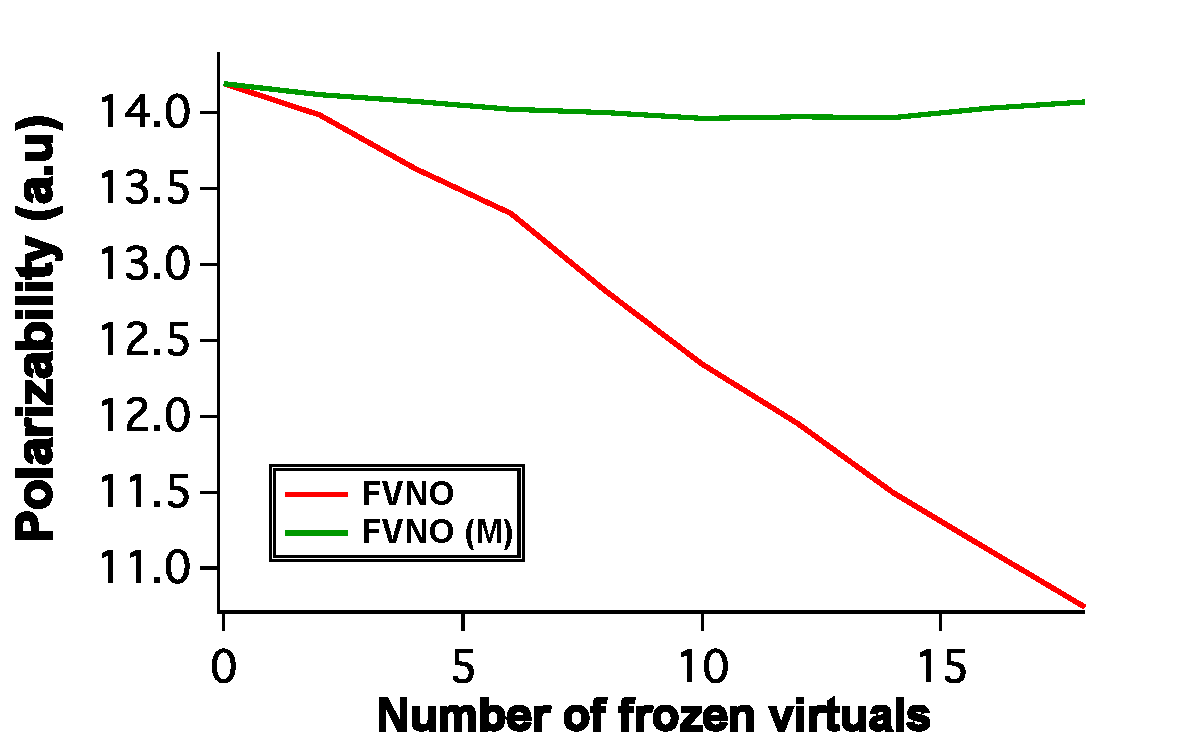
\includegraphics[width=0.6\linewidth]{figures_fvno++/fvno(m)_h2o2_adz_polar.pdf}
\caption{{\footnotesize CCSD/aDZ polarizabilities of
H$_2$O$_2$ in both FVNO and FVNO(M) schemes as a function of 
number of virtual orbitals removed.}}
\label{fig:fvno(m)_polar}
\end{MyFigure}
\begin{MyFigure}[h!]
\centering
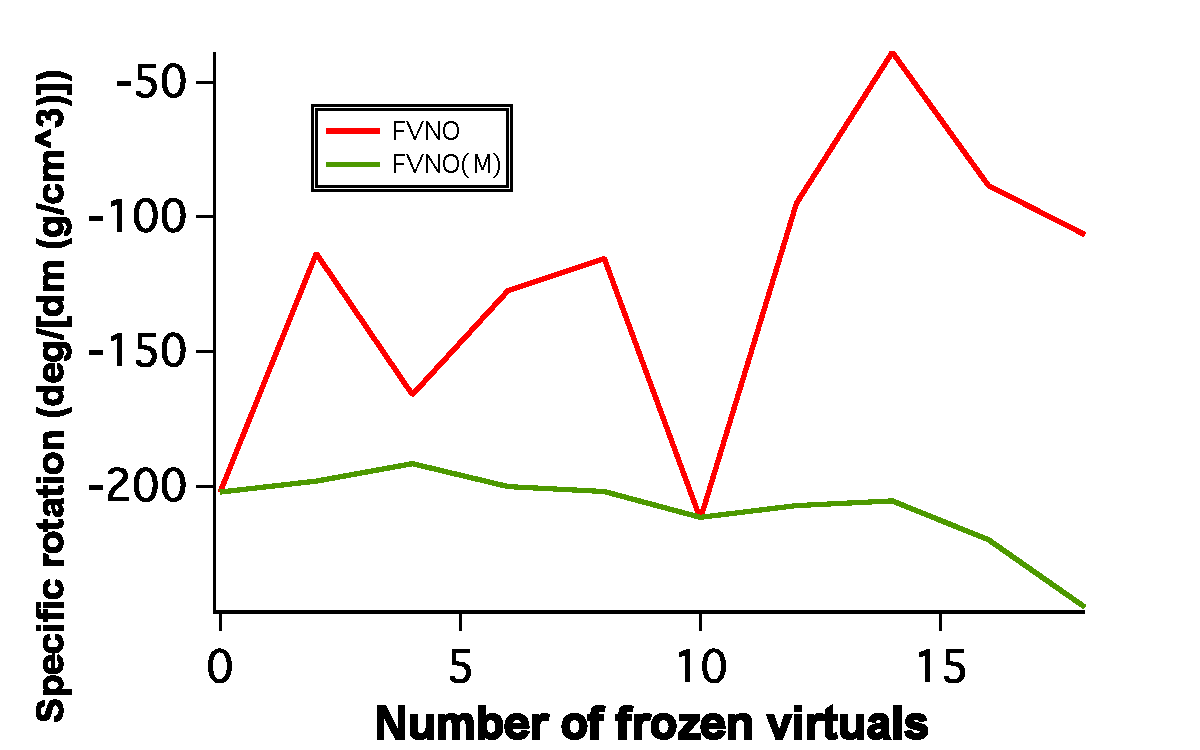
\includegraphics[width=0.6\linewidth]{figures_fvno++/fvno(m)_h2o2_adz_optrot.pdf}
\caption{{\footnotesize CCSD/aDZ/MVG specific rotations of
H$_2$O$_2$ in both FVNO and FVNO(M) schemes as a function of 
number of virtual orbitals removed.}}
\label{fig:fvno(m)_optrot}
\end{MyFigure}
compares the performance of this modified FVNO method (FVNO(M)) with the regular 
FVNO approach for calculating CCSD dynamic polarizabilities and specific rotations 
of the H$_2$O$_2$/aDZ system at 589 nm. Unsurprisingly, the errors in the FVNO(M) 
scheme are minimal compared to the original scheme for both polarozabilities and 
specific rotations even after 18 (out of 29) ``non-diffuse" VNOs are removed.
Specifically, the specific rotations curves are much well behaved in the 
FVNO(M) approach. The same behaviour can be expected for a majority of chiral molecules who 
like hydrogen peroxide require diffuse orbitals for a better description of the low lying 
Rydberg states. However, extension of this method to larger systems is not straightforward as OSEs are not a very robust 
crietria for selction of diffuse orbitals. Furthermore, not all diffuse orbitals 
are equally important for response properties. The FVNO++ scheme on the other
hand has a well-defined truncation criteria as the structure of the perturbed density
used in this approach closely resembles the response functions used to 
calculate these properties. Fig.~\ref{fig:fvno++_polar} 
\begin{MyFigure}[h!]
\centering
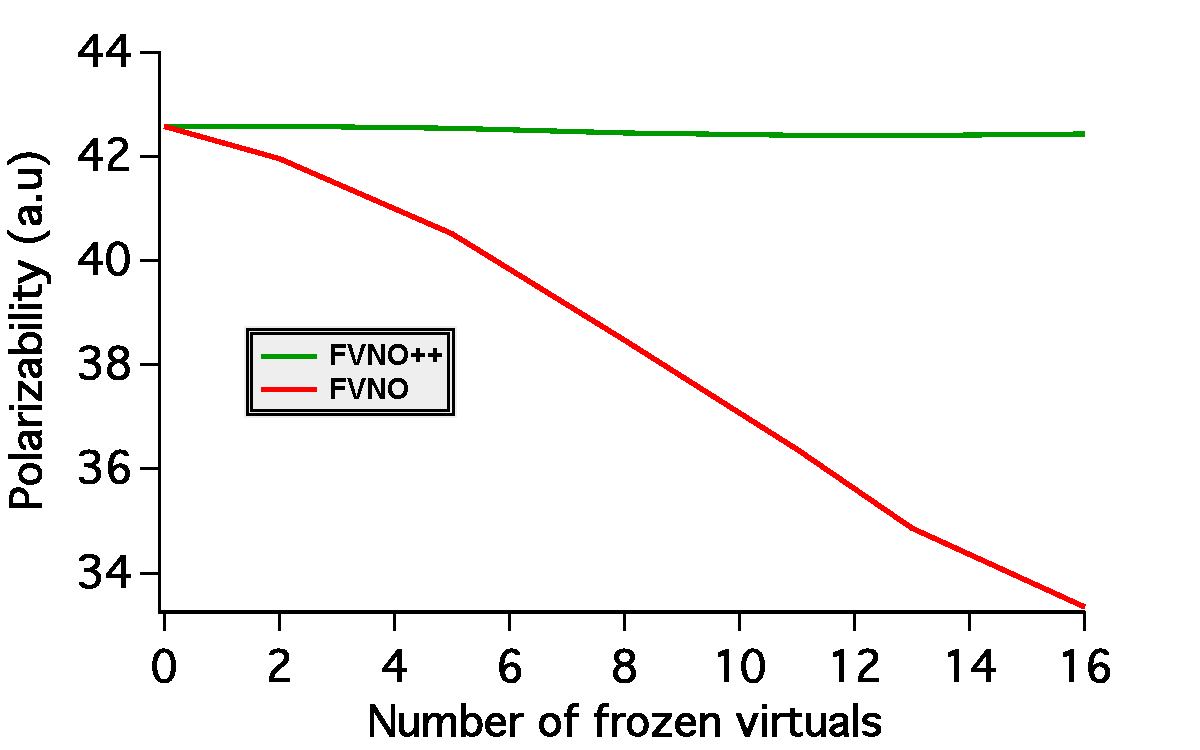
\includegraphics[width=0.6\linewidth]{figures_fvno++/fvno++_h2o2_adz_polar.pdf}
\caption{{\footnotesize CCSD/aDZ polarizabilities of
H$_2$O$_2$ in both FVNO and FVNO++($\mu$) schemes as a function of
number of virtual orbitals removed.}}
\label{fig:fvno++_polar}
\end{MyFigure}
compares the performance of both FVNO and electric dipole ($\mu$) based FVNO++ approach 
for calculating CCSD dynamic polarizabilities for the same system as above. It can be
easily seen that the FVNO++ scheme indeed captures the contribution of VNOs to
the response of the wavefunction. As a result, the removal of VNOs with low ONs
seem to have negligible effect on polarizabilities. Fig.~\ref{fig:fvno++_optrot}),
\begin{MyFigure}[h!]
\centering
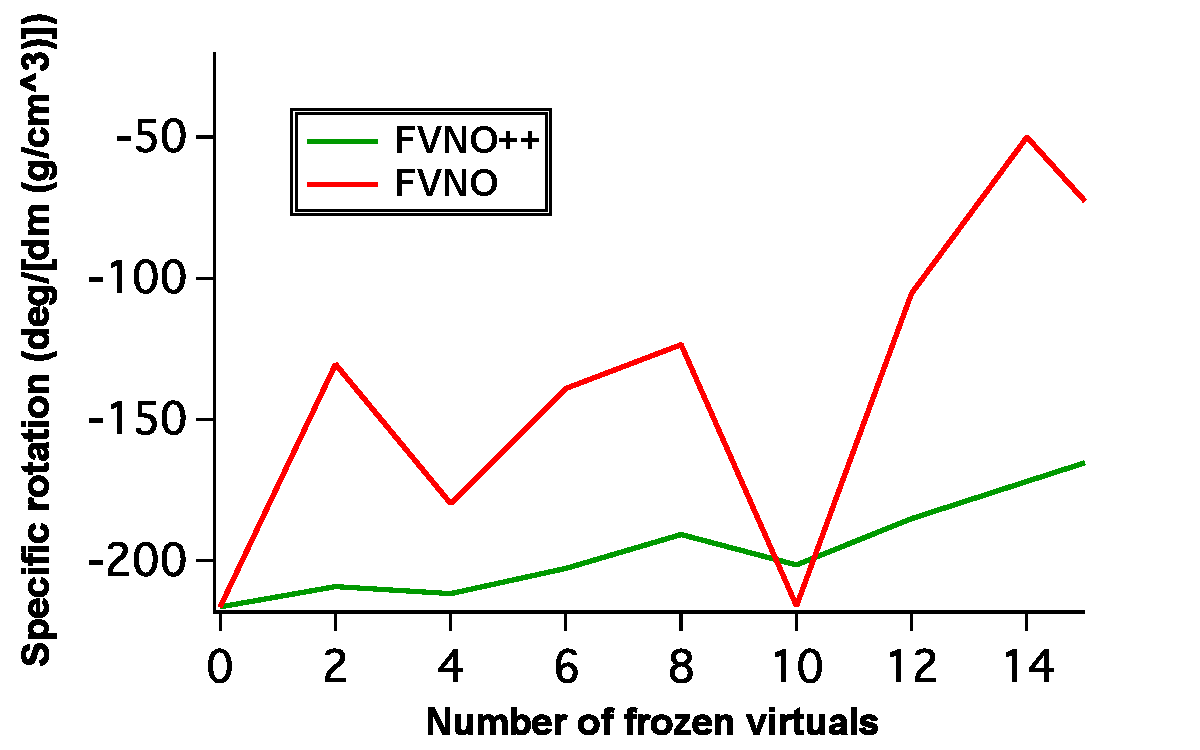
\includegraphics[width=0.6\linewidth]{figures_fvno++/fvno++_h2o2_adz_optrot.pdf}
\caption{{\footnotesize CCSD/aDZ/MVG specific rotations of
H$_2$O$_2$ in both FVNO and FVNO++($\mu$) schemes as a function of
number of virtual orbitals removed.}}
\label{fig:fvno++_optrot}
\end{MyFigure}
which plots the errors in the LG specific rotations in both FVNO and FVNO++($\mu$) schemes as VNOs
are removed, also shows similar trends. Specific rotations can be seen to be more 
sensitive than polarizabilities with respect to truncation of orbitals in both the methods.
However, the FVNO++ curve shows a systematic increase in error as more and more VNOs are
removed while the errors in the FVNO procedure are at best erratic.

%for large-scale calculations. Moreover, the metric of retention might
%be not well-defined. Thus, we instead look at the performance
%of the second-order perturbed density approach which we have named as FVNO++ 
%in the next sections.


%\subsection{$(H_2)_n$ Helices}
%- Linear structure, chiral, helical arrangement
%- best case for local correlation problems
%- small masses, high OR
%- Polariz, specific rotation (h2)4, (h2)5, (h2)6, (h2)7, maybe-bigger!! : LG, MVG, aDZ basis
%- diagnostics for FVNO++ approach:
%	- first comparing the structure of the ground state and perturbed density, one can see 
%	  that perturbed density would have a higher rank than ground-state density.
%	- how about incorporating L*L density as well and optimized NOs by better guess densities.
%	- Here we mostly concentrate on capturing the right kind of behavior rather 
%  	than savings, since there is not enough sparsity on offer for these cases.
%  	This is applicable for other test cases as well.

%\subsection{beta-pinene}
%\subsection{phenyl-ethanol}
%\subsection{norbornenone}
%Maybe bring MP2 diagnostics here as a reason for poor behavior! I mean here the pi-pi*
%excitations might require accurate T2 amplitudes as well.
%\subsection{Sparsity in solvated cluster}
\section{Conclusions}
We have developed a new formalism FVNO++ which offers a very 
compact representation of the virtual space for response 
property calculations. Based on plot studies on H$_2$O$_2$ using second-order 
electric dipole based perturbed densities, we conclude that this
approach has faster convergence towards the full canonical result for both 
polarizabilities and optical rotations than the original FVNO approach.
However, calculations with other choices of perturbed densities also need to be 
done, especially for bigger molecules to make the FVNO++ truncation scheme truly robust. 
We are currently in the process of a RI-CC2 linear response code\cite{} which we intend 
to use in conjunction with the FVNO++ formalism to tackle larger molecular systems.
Furthermore, we propose to extend this approach to the reduced-scaling techniques based 
on pair natural orbitals\cite{}.

%- Within the FVNO++ formalism, explored structures of second-order perturbed densities:
%Dab(2)(MU), Dab(2)(P), Dab(2)(MU,L), Dab2(P,L), Dab(2)(L) 
%employing different guesses of first-order perturbed amplitudes.  
%Based on plot studies on h2o2, we can conclude that 
%this approach works, has the right behavior/convergence properties.
%however, as usual, specific rotation is more sensitive than
%polarizabilities %and requires bigger virtual spaces.
%Future work: We also wish to report the sparsity pattern of the guess densities of large
%solvated molecular clusters using DF-MP2 which give us an estimate of
%the computational savings that can be exploited for such systems.
%Real application is solvated clusters, where we conclude that
%Hopefully, there is a lot of sparsity to take advantage of.
%\section{Acknowledgements}

